%% LyX 2.1.3 created this file.  For more info, see http://www.lyx.org/.
%% Do not edit unless you really know what you are doing.
\documentclass{article}
\usepackage[latin9]{inputenc}
\usepackage{color}
\usepackage{array}
\usepackage{verbatim}
\usepackage{booktabs}
\usepackage{amsmath}
\usepackage{graphicx}
\usepackage[authoryear]{natbib}

\makeatletter

%%%%%%%%%%%%%%%%%%%%%%%%%%%%%% LyX specific LaTeX commands.
%% Because html converters don't know tabularnewline
\providecommand{\tabularnewline}{\\}

%%%%%%%%%%%%%%%%%%%%%%%%%%%%%% User specified LaTeX commands.
% -----------------------------------------------
% Template for FMA2016
% (based on ISMIR 2010 Template)
% -----------------------------------------------
%
% To compile run:
% pdflatex fma2016template.tex
% bibtex fma2016template
% pdflatex fma2016template.tex (probably twice)
%
% requires the newapa Bibtex style

\usepackage{fma2016}
\setcitestyle{round}

% Title.
% ------
\title{Automatic Alignment of Long Syllables in A Cappella Beijing Opera}

% Single address
% To use with only one author or several with the _same address_
% ---------------
%\oneauthor
% {Author}
% {Affiliation \\ {\tt {author}@fma.edu}}
%
\oneauthor
 {Georgi Dzhambazov, Yile Yang, Rafael Caro Repetto, Xavier Serra}
 {Music Technology Group, Universitat Pompeu Fabra, Barcelona, Spain \\ {\tt \{georgi.dzhambazov, yile.yang, rafael.caro, xavier.serra\}@upf.edu}}
%
% Two addresses
% --------------
%\twoauthors
%  {First author, Second Author} {Affiliation1 \\ {\tt author1@fma.edu, author2@afm.edu}}
%  {Third author} {Affiliation2 \\ {\tt author3@fma.edu}}
%
% Three addresses
% --------------
%\threeauthors
%  {First author} {Affiliation1 \\ {\tt author1@fma.edu}}
%  {Second author} {Affiliation2 \\ {\tt author2@fma.edu}}
%  {Third author} {Affiliation3 \\ {\tt author3@fma.edu}}

\makeatother

\begin{document}
\maketitle 

\sloppy
\begin{abstract}
In this study we propose how to modify a standard approach for text-to-speech
alignment to apply in the case of alignment of lyrics and singing
voice.\textcolor{black}{{} We model phoneme durations by means of a
duration-explicit hidden Markov model (DHMM) phonetic recognizer based
on MFCCs}. The phoneme durations are empirically set in a probabilistic
way, based on prior knowledge about the lyrics structure and metric
principles, specific for the Beijing opera music tradition. \textcolor{black}{Phoneme
models are GMMs trained directly on a small corpus of annotated singing
voice.} The alignment is evaluated on a cappella material from Beijing
opera, which is characterized by its particularly long syllable durations.\textcolor{black}{{}
}Results show that the incorporation of music-specific knowledge results
in a very high alignment accuracy, outperforming significantly a baseline
HMM-based approach. 
\end{abstract}

\section{Introduction}

\begin{comment}
\textcolor{black}{LONG: Lyrics are one of the most important aspects
of vocal music. When a performance is heard, most listeners will fol-
low the lyrics of the main vocal melody. }
\end{comment}
{} \textcolor{black}{The task of lyrics synchronization (also known
as lyrics-to-audio alignment) has as an aim to find in an automatic
way a match between two representations of a musical composition:
the singing voice and the corresponding lyrics. Lyrics-to-audio alignment
may be used in various applications: for example to automatically
match structural sections from lyrics (verse, chorus) to a recording
of a particular singer. This facilitates navigation and can thus be
beneficial for musicologists or singing students.} 

\textcolor{black}{The problem of lyrics-to-audio alignment has inherent
relation to text-to-speech alignment. }Text-to-speech alignment has
been a research field for more than 20 years and thus yielded established
successful ways for modeling phonemes \citep{anguera2014audio}. However,
compared to speech, singing voice has some substantially different
characteristics including harmonics, pitch range, pronunciation, vibrato,
etc. In particular, unlike speech, for singing voice, durations of
vocals have on average somewhat higher variation \citep{kruspekeyword}.
This suggests that applying an approach from speech recognition out
of the box might not lead to satisfactory results. Traditional music,
characterized by frequent local tempo changes, poses an additional
challenge: Singers might prolong substantially certain syllables,
as a way to emphasize them or as an expressive singing element. 

Furthermore, current approaches on modeling lyrics are confined by
the necessity of a large speech corpus, on which phoneme models are
typically trained \citep{fujihara2012lyrics}. Such corpora might
not be present for every language or not freely available, as is the
case for Mandarin. %
\begin{comment}
 LONG: This is necessary because of the lack of a big enough annotated
training singing voice corpus. However this is rather cumbersome process
and requires a language-specific speech corpus. Furthermore 
\end{comment}
Recent work has shown that training on singing voice instead might
be a viable alternative \citep{hansen2012recognition}. 

In this paper we propose a lyrics-to-audio alignment method, which
relies on some of the specificities of lyrics structure of Beijing
opera as an additional cue to an appoach adopted from speech alignment.
One of the goals of the study is to show that enhancing computational
tasks with music-specific knowledge might improve accuracy.


\section{Background on Jingju music principles}

Lyrics in Jingju (also known as Beijing opera or Peking opera) come
from poetry and are thus commonly structured into couplets: each couplet
has two lyrics lines. A line is usually divided into 3 syllable groups:
a group is called \emph{dou} and consists of 2 to 4 written characters
\citep[Chapter III]{wichmann1991listening}\footnote{We use the\emph{ }term\emph{ syllable }as equivalent to one written
character. }. To emphasize the semantics of a phrase or according to the plot,
an actor has the option to sustain the vocal of the dou\textquoteright s
final syllable. In this work we will refer to the final syllable of
a \emph{dou }as \emph{key syllable.}

In addition to that, each aria from Jingju can be arranged into one
or more metrical pattern (called \emph{banshi}): it indicates the
mood of singing and is correlated to meter and tempo \citep{wichmann1991listening}.\textcolor{red}{{}
}\textcolor{black}{Usually an aria starts with a slow }\textcolor{black}{\emph{banshi,}}\textcolor{black}{{}
which gradually changes a couple of times to a faster one, to express
more intense mood. The language of Jingju is standard Mandarin with
some slight dialect.  }


\section{Related work}

\textcolor{black}{Current lyrics-to-audio alignment is mostly} based
on an approaches, adopted from text-to-speech alignment \citep{Mesaros96automaticalignment,fujihara2011lyricsynchronizer}:
A phonetic recognizer is built from speech corpus, whereby a hidden
Markov model (HMM) is trained for each phoneme. The acoustics of phonemes
are described by mel frequency cepstral coefficients (MFCCs). In an
example of such an approach, polyphonic Japanese and English pop music
is aligned \citep{fujihara2011lyricsynchronizer}. The authors propose
to adapt the speech phoneme models to the specific acoustics of singing
voice by means of Maximum Likelihood Linear Regression. This is necessary
because of the lack of a big enough singing voice corpus for training.
Further, an automatic segregation of the vocal line is performed,
in order to reduce the spectral content from background instruments. 

HMMs, being originally applied to model spoken phonemes,  have the
drawback that, in general, are not capable to represent well vowels
with long and highly-variable durations. This is because the waiting
time in a state in traditional HMMs cannot be unlimitedly long \citep{rabiner1989tutorial}.
Durations can be modeled instead by \textcolor{black}{a duration-explicit
hidden Markov model (DHMM)} (also known as hidden semi-Markov model).
In DHMMs the underlying process is allowed to be a semi-Markov chain
with variable duration of each state \citep{yu2010hidden}. DHMMs
have been applied to detect keywords from a cappella English pop songs
\citep{kruspe2015keyword}. The author showed that accuracy of detection
increases if the duration of each phoneme is learned from a singing
dataset. In addition, DHMMs have been shown to be successful for modeling
other problems from the domain of music information retrieval: They
have been, for example successful in representing chord durations
in automatic chord recognition \citep{chen2012chord}.

To our knowledge, very few studies of lyrics-to-audio alignment have
been conducted on songs with Chinese language, as an example on Cantonese
Chinese \textcolor{black}{\citep{wong2007automatic}.} %
\begin{comment}
\textcolor{black}{LONG RELATED WORK: }

Very few works have trained models directly from singing voice: \textcolor{red}{add
from YILE: Anna Kruspe, Hansen, }ADD Kruspe: songified.
\end{comment}



\section{Approach overview}

\textcolor{black}{To model phoneme durations, we rely on a DHMM}\footnote{\textcolor{black}{For brevity in the rest of the paper the proposed
alignment scheme will be referred to as DHMM.} }\textcolor{black}{.} A general overview of the proposed approach is
presented in Figure \ref{approach overview}. First an audio recording
of an aria is manually divided into audio segments corresponding to
lyrics lines as indicated in the lyrics script of the aria, whereby
instrumental-only sections are discarded. All further steps are performed
on each line segment of audio. If we had used automatic segmentation
instead, potential erroneous lyrics and features could have biased
the comparison of a baseline system and DHMM. As we focus on evaluating
the effect of DHMM, manual segmentation is preferred. %
\begin{comment}
Lyrics are read from TextGrid annotation layer 'lines' IMPL: lyricsParser.divideIntoSectionsFromAnno
\end{comment}


Then each lyrics line is expanded to a sequence of phonemes, whereby
reference syllable durations guide the alignment process. The main
contribution of this work is twofold: 1) the application of music-specific
rules for the creation of reference durations and 2) training phonemes
on singing voice.

\begin{figure}
\begin{raggedright}
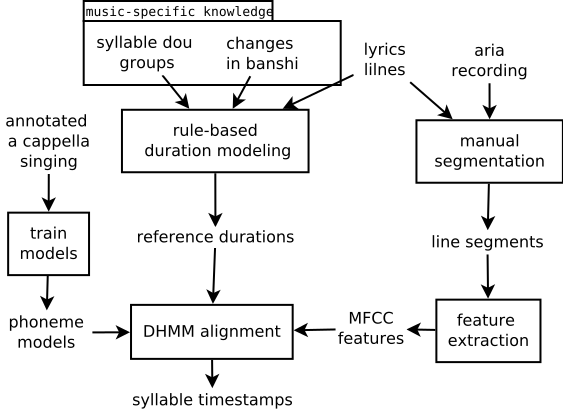
\includegraphics[width=0.95\columnwidth]{systemOverview}
\par\end{raggedright}

\protect\caption{Approach Overview: The middle column shows how reference durations
are derived based on music-specific knowledge.}
\label{approach overview}
\end{figure}
\begin{figure*}[!t]
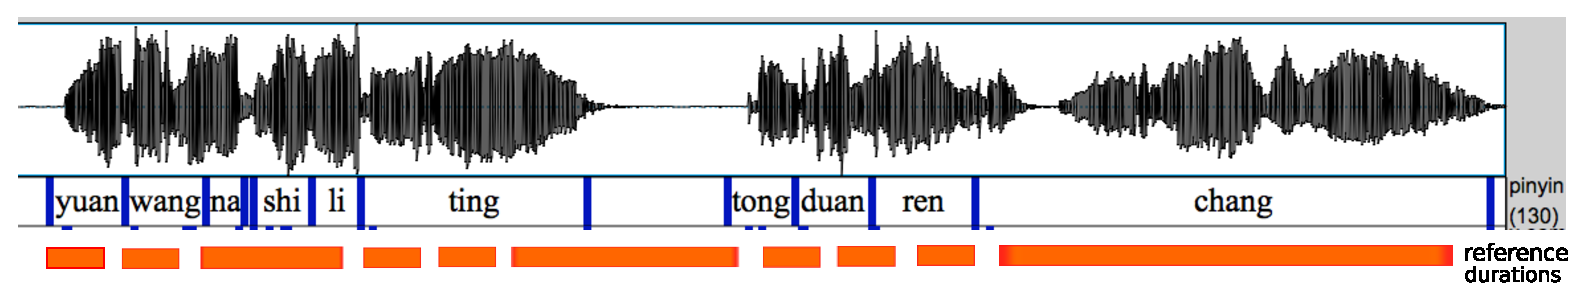
\includegraphics[width=0.9\paperwidth]{praat_annotation_sentence_refDurs}

\protect\caption{An example of 10-syllable line, being last in a \emph{banshi} (before
the \emph{banshi} changes). Actual syllable durations are in pinyin,
whereas reference durations are in orange parallelograms (below).}
\label{example}
\end{figure*}



\subsection{Rule-based duration modeling}

The idea of the duration modeling is that the actual duration of a
phoneme can be seen as being generated by a statistical distribution
with highest probability at an expected reference duration. The reference
durations can be assigned using any prior knowledge like for example
structure of lyrics segments, as has been done by \citet{wang2004lyrically}.
In this work they are derived as follows: 

Firstly,\emph{ }each \emph{key syllable }in\emph{ }a \emph{dou} is
assigned longer reference duration according to empirically found
ratios, while the rest get equal durations.%
\begin{comment}
IMPL: in SentenceJingju.SentenceJingju.assignReferenceDurations()
\end{comment}
{} Additionally, we observed in the dataset that usually the last \emph{key
syllable} of the last line in a \emph{banshi} is prolonged additionally.
Thus we lengthened additionally the reference syllable duration of
these last \emph{key syllables. }Figure \ref{example} depicts an
example. According to \emph{dou} groups the 3rd, 6th and last syllable
are expected to be prolonged. Note that for the example this expectation
does not hold for the 3rd syllable.

Then, to form a sequence of phoneme reference durations $R_{i}$,
the reference durations of syllables are divided among their constituent
phonemes, according to the initial-middle-final division of syllables
in Mandarin \citep{duanmu2000phonology}. %
\begin{comment}
LONG: Another complication are the dphtongs and triphtong syllables
in the language.
\end{comment}
A syllable has a middle part (nucleus) being a simple vowel, a diphthong,
or triphthong. An initial part (a consonant) or a final part (a group
of consonants) is optional. We assign consonants a fixed reference
duration $R_{c}=0.3$ seconds, while the rest of the syllable is distributed
equally among vowels. %
\begin{comment}
consonant duration is fixed. ParametersAlgo.CONSONANT\_DURATION. see
IMPL: jingju.SyllableJingju.SyllableJingju.calcPhonemeDurations
\end{comment}
\textcolor{black}{The reference durations $R_{i}$ are linearly scaled
to a reference number of frames according to the ratio between the
number of phonemes in a lyrics line and the duration of its corresponding
audio segment.}


\subsection{Phoneme models}

For each phoneme a GMM is trained on annotated a cappella singing.
The first 13 \textcolor{black}{MFCCs} and their \ensuremath{\Delta}
and \ensuremath{\Delta}\ensuremath{\Delta} are extracted from 25ms
audio frames with the hop size of 10ms. The extracted features are
then fit into a phoneme GMM with 40 components: a number of components
usually proved as sufficient in speech recognition. A model for silent
pause \emph{sp} is added at the end of each syllable, which is optional
on decoding. This allows to accommodate the frequent for Jingju regions
of pauses after some syllables.


\subsection{DHMM alignment\label{sub:DHMM}}

\begin{comment}
IMPL: SyllableJingju.SyllableJingju.calcPhonemeDurations

sp at end of syllables are not optional. They are assigned duration
as a consonant A, which might result in actual duration from 0 to
A 
\end{comment}


The syllables for a line are expanded to a sequence of phonemes based
on grapheme-to-phoneme rules \footnote{We built a pinyin-to-X-Sampa mapping available at https://github.com/georgid/AlignmentDuration/blob/noteOnsets/jingju/syl2ph.txt}.
Then the trained GMMs are concatenated into a phonemes network, represented
by a HMM, where each GMM is a state. The HMM is aligned to the MFCC
features, extracted from the aria, being aligned. The most likely
state sequence is found by means of a forced alignment with Viterbi
decoding.

\textcolor{black}{We have adopted the idea of \citet{chen2012chord}
not to represent durations by an additional counter state in the HMM,
but instead to modify the Viterbi decoding stage}. Let us define
\begin{description}
\item [{$\delta_{t}(i):$}] probability for the path with highest probability
ending in state \emph{i} at time \emph{t} (comply with the notation
of \citet[III. B]{rabiner1989tutorial})) 
\end{description}
Now maximization is carried over the most likely duration for each
state, instead of over different states:

\begin{equation}
\delta_{t}(i)=\max_{d}\{\delta_{t-d}(i-1)\thinspace P_{i}(d)\thinspace[B_{t}(i,d)]\}\label{eq:decoding}
\end{equation}
\begin{comment}
Alpha=0.97, maybe it should be tested with diff alpha
\end{comment}


where $B_{t}(i,d)$ is the observation probability of staying $d$
frames in state $i$ until frame $t$. \textcolor{black}{The duration
$d$ of a phoneme is modeled as a normal distribution ${\cal N}\sim(R_{i};\sigma)$,
with a peak at $R_{i}$. }Thus, we chose to restrict the domain of
$d$ to $(\max\{R_{i}-\sigma,1\},R_{i}+\sigma)$. Note that in forced
alignment the source state could be only the previous state $i-1$.
\textcolor{black}{More details on the inference with DHMM can be found
in our previous work \citet{Dzhambazov}. In comparison to our previous
work, we opted for dividing the global standard deviation $\sigma$
into $\sigma_{c}$ for consonants and $\sigma_{v}$ for vowels. Proper
values for $\sigma_{c}$ and $\sigma_{v}$ assure that a phoneme sung
longer or shorter than the expected $R_{i}$ can be adequately handled.
Another modification we did is that $sp$ models are assigned an exponential
distribution, because the duration of inter-syllable silences cannot
be predicted. }%
\begin{comment}
\textcolor{black}{IMPL: distribution type set in align.\_LyricsWithModelsBase.\_LyricsWithModelsBase.\_phonemes2stateNetwork.
maximum constant duration in ParametersAlgo.GLOBAL\_WAIT\_PROB.}
\end{comment}



\section{Dataset\label{sec:Dataset}}

The dataset has been especially compiled for this study and consists
of excerpts from 15 arias of two female singers, chosen from a \emph{CompMusic
}corpus of Jingju arias \citep{repetto2014creating}. For a given
aria were present two versions: a recording with voice plus accompaniment
and an accompaniment-only one. Thus a cappella singing was generated
by subtracting the instrumental accompaniment from the complete version\footnote{The resulting monophonic singing is as clean as if it were a cappella,
having slightly audible artefacts from percussion on the non-vocal
regions}. Table \ref{dataset_stats} presents the average values for lines
and syllables.
\begin{table}
\begin{centering}
\begin{tabular}{cc>{\centering}p{0.2\columnwidth}}
\toprule 
 & dataset & 'canonical' dataset\tabularnewline
\midrule 
\textbf{duration (minutes)} & 67 & 27\tabularnewline
\midrule 
\textbf{\#lines per aria} & 9.2 & 9.9\tabularnewline
\midrule 
\textbf{\#syllables per line} & 10.7 & 10.3\tabularnewline
\midrule 
\textbf{line duration (seconds)} & 18.3  & 23.4\tabularnewline
\midrule
\textbf{syllable duration (seconds)} & 2.4 & 3.1\tabularnewline
\bottomrule
\end{tabular}
\par\end{centering}

\protect\caption{Line and syllable averages about the dataset}
\label{dataset_stats}
\end{table}


Each aria is annotated on the phoneme level by native Chinese speakers
and a Jingju musicologist. The phoneme set has 29 phonemes and is
derived from Chinese pinyin, and represented using the X-sampa standard\footnote{Annotations are made available at http://compmusic.upf.edu/node/286}.
To assure enough training data for each model, certain phonemes are
grouped into phonetic classes, based on their perceptual similarity. 

Further, we selected a 'canonical' subset of the dataset, consisting
of lines, according to the assumptions we made: \emph{key syllables}
should be prolonged. Thus, we kept only these audio segments, for
which at most one \emph{key syllable} is not prolonged and discarded
the rest. We considered a syllable as being prolonged if it is longer
than 130\% of the average syllable duration for the current line.
\begin{comment}
IMPL: isNonKeySyllLong is annotated in Praat with 1 or 0 and is a
field in jingju.SectionLinkJingju.SectionLinkJingju
\end{comment}



\section{Experiments}

Alignment accuracy is evaluated as the percentage of duration of correctly
aligned syllables from total audio duration (see \citet[figure 9]{fujihara2011lyricsynchronizer}
for an example). Accuracy is measured for each manually segmented
line and accumulated on total for all the recordings\footnote{To encourage reproducibility of this research an efficient open-source
implementation together with documentation is available at https://github.com/georgid/AlignmentDuration/tree/noteOnsets/jingju.}.


\subsection{Experiment 1: oracle durations}

To define a glass ceiling accuracy, alignment was performed considering
phoneme annotations as an oracle for acoustic features. Looking at
phoneme annotations, we set the probability of a phoneme to 1 during
its time interval and 0 otherwise. We found that the accuracy per
line of lyrics is close to 100\%, which means that the model is generally
capable of handling the highly-varying vocal durations of Jingju singing.
Most optimal results were obtained with $\sigma_{c}$ = 0.7 seconds;
$\sigma_{v}$ = 2.0 seconds, which are used in experiment 2. %
\begin{comment}
done by setting parameter withOracle in doitOneChunkAlign.doitOneChunkAlign

For each state for a phoneme, for the frames of its duration assign
1 in B\_map. So B\_map is zero for all other phonemes. 
\end{comment}
{} %
\begin{comment}
if phoneme is not present in model, approximate by copying the model
for a closely sounding phoneme.

``missing'' -> ``replace by''

U\textasciicircum{} -> copy u

@ -> copy e

9 -> copy O

----

for these since capital letters are used, they dont make difference
when loading .pkl files.

N -> copy n

A -> copy a

o -> copy O
\end{comment}



\subsection{Experiment 2: comparison with baseline}

As a baseline we employ a standard Viterbi decoding, run with the
\emph{htk} toolkit \citep{young1993htk}. For both baseline and DHMM,
to assure good generalization of results, evaluation is done by cross
validation on 3 folds with approximately equal number of syllables:\textcolor{green}{{}
}\textcolor{black}{Phoneme models are trained on 10 of the arias using
the phoneme-level annotations and evaluated on a 5-aria hold-out subset}.We
have further evaluated on the 'canonical' selected subset of lyrics
lines, introduced in Section 5. Table \ref{results} shows that the
proposed duration model outperforms significantly the baseline alignment.
The improved accuracy for 'canonical' lyric lines can be attributed
to the increased degree, to which prior duration expectations are
met. \textcolor{red}{}%
\begin{comment}
always set align.ParametersAlgo.ParametersAlgo.WITH\_SHORT\_PAUSES
= 1 for Jingju
\end{comment}



\section{Conclusion}

In this work we evaluated the behavior of a HMM-based phonetic recognizer
for lyrics-to-audio alignment in two settings: with and without utilizing
lyrics duration information. Using probabilistic duration-explicit
modeling of phonemes for the former setting outperformed the latter
on recordings of a cappella Beijing opera. It has incorporated prior
expectations of syllable durations, based on knowledge specific for
this music genre. In particular, the proposed DHMM aligns remarkably
well a selected set of lyrics lines, which comply more precisely with
these music-specific principles.
\begin{table}
\noindent \begin{centering}
\begin{tabular}{cccc}
\toprule 
 & baseline & DHMM & oracle\tabularnewline
\midrule
\textbf{overall} & 56.6 & 89.9 & 98.5\tabularnewline
\midrule 
\textbf{'canonical'} & 57.2 & 96.3 & 99.5\tabularnewline
\bottomrule
\end{tabular}
\par\end{centering}

\protect\caption{Comparison of accuracy on oracle, baseline and DHMM alignment on total
and selected arias. Accuracy is reported as accumulate correct duration
over accumulate total duration over all lines from a set of arias.}
\label{results}

\begin{comment}
IMPL: run with commit: https://github.com/georgid/JingjuAlignment/commit/87e593d2c32c6a385c69691370f2bb8ee77328cf

see comments of commit in github

----

baseline is with htk. So it has silence model and the one hiere does
not. So include it in paper.
\end{comment}
\end{table}
\begin{comment}
LONG: In Figure \ref{comparison-one-aria} is depicted the model's
accuracy for an aria with very long \emph{key syllables}, for which
the baseline model performs poor, whereas the DHMM aligns decently
\footnote{Please find attached a video recording demonstrating the alignment
accuracy}. One can see the advantage of the proposed model for example for
lyrics line 5. 
\begin{figure}
\includegraphics[width=1\columnwidth]{figure_Accuracy_xixiangji_biuntian.png}

\protect\caption{Comparison of oracle, baseline and DHMM results on one aria. Each
point represents one lyrics line, vertical lines represent \emph{banshi}
changes }
\label{comparison-one-aria}
\end{figure}
\end{comment}



\subparagraph*{Acknowledgements}

\textcolor{black}{We are thankful to Wanglei from }\textcolor{black}{\emph{Doreso}}\textcolor{black}{{}
for providing a dictionary of pinyin syllables.}\textcolor{red}{{} }This
work is partly supported by the European Research Council under the
European Union\textquoteright s Seventh Framework Program, as part
of the CompMusic project (ERC grant agreement 267583) and partly by
the AGAUR research grant.

\bibliographystyle{plainnat}
\bibliography{JingjuAlignment,/Users/joro/Documents/Phd/UPF/voxforge/myScripts/AlignmentDuration/ISMIR_noteOnsets/JabRefOnsetDetectionFullReferences}

\end{document}
